% !TEX root = thesis.tex
\chapter{深層学習の実装における課題とその対策の提案}
この章では、まず深層学習のアルゴリズムを実装する際に起こり得る、3つの問題点について整理する。次に、3つの問題点を解決するため、開発者が採ることの出来る対策について詳しく考察する。考察の一部では、実際のソースコードによる実証実験が必要となる。この実験については、5章にて詳しく述べる。

\section{深層学習の実装における問題点}
深層学習のアルゴリズムを、ウェブ工学などに応用するための具体的な実装を行う際の問題点として、次の3つの問題が考えられる。
\begin{itemize}
\item \textbf{分類精度の再現の問題}。 深層学習が注目された大きな理由である、高い識別精度を実現できるアルゴリズムかどうか。また、論文において掲げられている精度を再現できる実装を手元に用意したり、あるいは制作できるかどうか。
\item \textbf{実装難易度の問題}。実際の問題に応用するにあたって、必要なプログラミング技術や数学的知識は、出来るだけ低くて済む方が望ましい。
\item \textbf{学習時間の問題}。深層学習では、 学習にかかる時間が非常に長くなることがある。グラフィックスプロセッシングユニット(Graphics Processing Unit、以下GPU)を用いることで実行速度を上げることが出来るが、GPUを利用するための実装自体も難しい。これは、実装難易度の問題とも関連する。
\end{itemize}
以下、これら3つの問題について、詳しく述べる。

\subsection{分類精度の再現の問題}
今回深層学習を選択した理由は、ウェブ工学のタスクにおいて、高い分類精度を実現するための最も有力な方法だと思われるからである。逆に、深層学習の分類精度が従来の分類器より劣っているならば、従来の分類器を使った方が望ましいと言える。\par
アルゴリズムを紹介する論文では、対応する実装が公開されていなかったり、例えメインのアルゴリズムについては書いてあっても、実験の際に設定したハイパーパラメータの詳細について記していない場合がある。ハイパーパラメータの値や決め方が公開されていない場合、自ら全てのコードを実装したり、問題に応じてアルゴリズムの細部やハイパーパラメータを柔軟に調整しなければならない場合もある。利用者が実装したり手を加えたソースコードでは、論文の著者と正確に同じモデルやアルゴリズムを使用できているのかどうかが不明である。よって、本当に論文に記述してある性能が発揮できるのかどうか、実際に利用してみないとわからない。この問題は、論文で扱っていない新しい入力データを扱う場合により顕著になると考えられる。なぜなら、初めてのデータにおいては、仮に論文のものと細部まで等しいアルゴリズムを実装できたとき、どの位の分類精度が実現できるのかわかっていないため、アルゴリズムの精度面での正しさを検証することが出来ないからである。\par

\subsection{実装難易度の問題}
この問題は、主に標準といえる公開ライブラリが確立していないことが原因である。深層学習は歴史の浅い発展途上の技術であり、どのアルゴリズムを定番とすれば良いのか、試行錯誤の段階にある。各アルゴリズムの改良点が次々と見つかっていることに加え、学習性能が高くなる原理や、学習対象に対する各アルゴリズムの得手不得手など、解明中の部分も多い。アルゴリズムが開発途上で確定できていないため、公開されているライブラリも、現状では、開発用途や実験的なものが多くなってしまっている。実験的なライブラリでは、一部の種類のデータに対する学習のみを想定している場合があり、この場合他の種類のデータを扱うためには、データ変換用のソースコードを記述しなければならない。\par%標準ライブラリがある分野、例えばLIBSVMやmatlabの制御系、excelの統計は利用が簡単なことに言及
手元のパソコンにて実行可能な深層学習のソースを探し当てたとしても、このソースが実際に、論文にて示されているような高い精度を実現できるかどうかは、実際のデータを当てはめてみるまで定かではない。これは先ほど述べてように、まだアルゴリズムの細部が固まっておらず、実装ごとにバリエーションが大きいためである。また、ソースコードが言わばお試し用の状態になっていて、単にアルゴリズムの要点を示すためのものだったり、実行時間の短縮を重視したハイパーパラメータの調整が為されていて、論文に記述してある精度を実現できないこともある。\par
このようにライブラリが確立していない状況では、プログラマが自ら深層学習のコードを記述する必要がある。しかし、深層学習の原理は多くの数学的背景の下成り立っており、理解には多くの時間がかかる。結果としては、プログラム開発に長い時間がかかってしまい、ビジネスシーンにおいて不利であると考えられる。なおライブラリの未成熟さや、実装・改造の難しさは、自力実装における「分類精度の再現の問題」にも影響している。\par

\subsection{学習時間の問題}
深層学習のモデルを訓練するには、無視できない長さの時間が必要となる。例えば、先述したGoogleによるSupervisionの学習では、1000台のマシンによるクラスタを用いても、訓練に3日間かかっており、個人レベルでは実験自体がほぼ不可能である\cite{le2012building}。一回の学習の時間が長くなれば、それだけ技術開発にかかる時間も長くなり、刻一刻と変化するウェブサービスに対して応用するのは難しくなる。特に、スタートアップ企業が深層学習の技術を用いて市場での優位を得ようとする場合を考えると、開発期間の短縮は大きなポイントである\cite{ries2011the-lean}。\par
必要実行時間の長さをカバーするため、GPUを用いて演算をスピードアップさせる手法が確立されつつあるが、GPUは比較的高価なパーツである上、GPUの利用には特殊なプログラミングが要求され、開発における障壁の1つとなっている(つまりこれは「実装難易度の問題」でもある)。また、大部分のノートパソコンや一部のサーバなど、並列演算に利用可能なGPUの搭載自体が出来ないパソコンを使っている場合ではGPUを利用しているソースコードの実行が全く出来ないこともある(後述)。\par

この章の残りでは、今挙げた「分類精度の再現の問題」「実装難易度の問題」「学習時間の問題」を解決するための方策について述べる。ただし、「分類精度の再現の問題」については、最終的にソースコードを実行してみないと、再現性が確保されていることを確かめられない。そこで、「分類精度の再現の問題」については、5章にていくつかのアルゴリズムや実装による実験を行うことで、更なる検証を行う。

\section{実装上の問題への対策}
ここでは、前節で述べた3つの実装における問題点のそれぞれに対して、開発者がどのような対策を採れるのか、考察する。また、これらの3つの問題点の全てに共通して、「適切なライブラリの組み合わせを選択する」という対策が有効である。これについては、最後にまとめて言及する。

\subsection{分類精度の再現の問題への対策}
\label{subsec:c4_provision_replication}
「分類精度の再現の問題」は、論文だけでは実装に必要な全ての情報が得られないことが原因である。これを解決する最も簡単な手段は、論文やアルゴリズムの中で、実際に分類実験に用いたソースコードをそのまま提供しているものを選び、そのソースコードを出来るだけ変更せずに使うことである。

深層学習のプログラムを実装するために、まず大きく分けて、「自分でソースコードを全て書く」方法と、「主に既存のソースコードを利用する」方法の2つが考えられる。「既存のソースコードを利用する」場合のメリットとして、
\begin{itemize}
\item 開発時間が大きく短縮され、バグも起こりにくい。選考論文のみをたよりにゼロから実装を行うと、時間がかかる上、バグが混入する危険性も高い。
\item 論文では省略された僅かな実装ノウハウの差により、性能が低下してしまう危険性を、排除できる。
\item メジャーな実装をベースにすれば、改造部分も利用してもらいやすくなる。
\end{itemize}
という点が挙げられる。デメリットとしては、
\begin{itemize}
\item 使っているソースコードが、本当に深層学習のアルゴリズム・実装として、信頼できるのかわからない。
\item 始めのうちはソースコード中に、内容が理解できないブラックボックス部分が増えてしまうため、改造にかかる時間が長くなる。 改造に留まらず全く新しいアルゴリズムを実装する場合、ゼロからスタートした方が、元ライブラリの制約に縛られずに早く書けるケースもある。
\end{itemize}

などの要素が想定される。しかし、分類精度を再現できる可能性を高くするため、今回は既存のソースコードを探して利用していくことにした。既存ソースコードを利用する際に生じるリスクについては、図\ref{c4_library_hedge}のように対処できる。まず、実装の信頼性については、精度の再現実験を行うことで担保する。実装の自分がチェックしていない部分で何が行われているかはわからないが、ひとまず深層学習に期待される精度を再現してくれるソースコードであれば、深層学習の正当なアルゴリズムとしてひとまず認めてしまおうという考え方である。次に、改良が難しくなる問題については、出来るだけドキュメントやソースコード中のコメントが整備されており、ライブラリ全体の構成も使いやすく読みやすいものを選ぶ。また、学習の過程や結果を可視化することで、内部処理についての理解を深めやすくなる。\par

\begin{figure}[tbp]
 \begin{center}
  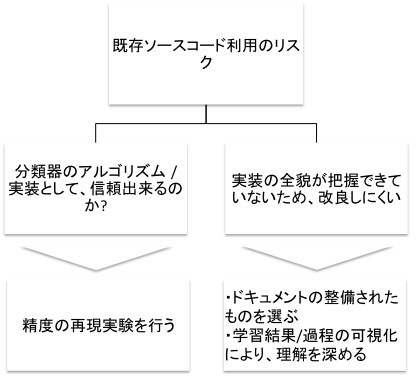
\includegraphics[width=90mm]{img/c4/library_hedge}
 \end{center}
 \caption{既存ソースコード利用のリスクと、対処方法}
 \label{c4_library_hedge}
\end{figure}
なお、「自分でソースコードを全て書く」場合のメリットとデメリットは、上記「既存のソースコード」の場合の逆となる。自分で新たなコードを書くので時間がかかり、バグの混入リスクも大きい。また、ソースコードを公開した場合の、ライブラリとしての信頼度も、ゼロから築かなければならない。ただし、深層学習の新たなアルゴリズムを開発する段階に至った研究者にとっては、既存のソースコードの細部を改造するよりも、全て自分の手で書いたコードを使う方が、より深い理解を得やすく、確実で素早い実装ができる可能性もある。

\subsection{実装難易度の問題への対策}
\label{subsec:c4_provision_difficulty}
「分類精度の再現の問題」でも挙げた、既存のソースコードを利用することが、「実装難易度の問題」に対する直接的な解決方法の1つにもなる。深層学習のアルゴリズム自体が改良の過程で単純な数学的モデルへと帰着し、実装が容易になる可能性も否定できないが、ここでは現段階で採れる方策のみを考えるということで、除外する。\par
ただし、実装難易度を下げるという観点からは、「分類精度の再現の問題」を解決できるだけでなく、さらにソースコードの利用や解読・改造が容易であることが重要である。ソースコードの改造については、もちろん全くしないで済むのが理想ではある。しかし実際には、現在の深層学習のアルゴリズムで、細部の調整なしに良い結果を出すことは難しい。よって応用開発ではいくらかのプログラミングが必要となることが予想される。このときソースコードの読みやすさや改造のしやすさは重要な長所となる。また、ソースコード開発コミュニティが活発であれば、自分以外の開発者がソースコードの問題点やバグを修正してくれる可能性が出てくる。開発上で生まれた疑問が、コミュニティの構成員によって解決してもらえることもあるため、実装の助けとなる。\par%オープンソース
深層学習に利用できるライブラリは、まだ標準が固まっていないものの、論文と共にソースコードを公開するパターンが多く、いくつか出回っている。\ref{sec:c4_deep_library}ではどのようなライブラリが存在するかについて詳しく述べると共に、今回の問題点を解決する上では、Pylearn2というライブラリを用いることが最も適切だと示す。


\subsection{学習時間の問題への対策}
\label{subsec:c4_provision_exectime}
学習時間を短縮するためには、アルゴリズム自体の改良が最も重要であるが、もちろんその難易度は高い。ここでは、アルゴリズムを実行するハードウェアに着目し、特に近年盛んになっているGPUの利用による高速演算、GPUコンピューティングに焦点を当てる。
\subsubsection{GPUの利用による高速化}
GPUとは、CPUと併用できるプロセッサの一種で、主に画像処理演算を担当している。GPUは元々、画像処理に必要な行列演算などを、CPUよりも効率良く扱えるように開発された。現代のGPUは、単にグラフィック処理に特化したプロセッサというだけでなく、その並列演算能力を活かして、大量の演算を行う科学計算用途にも使われている。GPU設計・製作メーカーのNVIDIAからは、グラフィック出力機能を敢えて外し、科学計算用途に特化した、TeslaというハイエンドGPUシリーズも発売されている\footnote{\url{http://www.nvidia.co.jp/object/tesla-supercomputing-solutions-jp.html}}。\par 
深層学習の研究においても、GPUによる並列計算が有効とされている。これは、入力ベクトルと重み行列の積など、ニューラルネットワークの計算にて中心を占める行列演算が、並列計算の恩恵を受けやすいからである\cite{bengio2012practical}。例えば、前述したDropConnectの研究\cite{wan2013regularization}に拠れば、GPUで演算した場合、テクスチャメモリを利用しなくてもCPUより97.2倍高速化でき、テクスチャメモリを利用すれば414.8倍の速度を出すことも可能である。\par
また、深層学習の実装によっては、はじめからGPUで高速化することを前提に、GPU専用のコードを書いている場合がある。例えば、後述するcuda-convnet\footnote{\url{https://code.google.com/p/cuda-convnet/}}や、Maxout Network\cite{goodfellow2013maxout}のコードの一部、DropConnect\cite{wan2013regularization}\footnote{\url{http://cs.nyu.edu/~wanli/dropc/}}が該当する。この場合、そもそもGPUを搭載したマシンを使わないと、コンパイルや実行が全く出来なくなってしまう。\par
%CPUの計算能力は頭打ちになっている。
GPUが高速に演算を実行できる理由は、その構造にある。1〜数個のプロセッサで様々な命令をこなすCPUに対し、GPUは数百〜数千個のcoreを持っており、同一の命令を高速に並列演算する用途に向いている。これは、大量の点の変換処理が必要となるグラフィック処理環境から生まれたGPUの強みである。かつてGPUを科学演算に用いるには、OpenGL\footnote{\url{http://www.opengl.org/}}やCg\footnote{\url{http://www.nvidia.co.jp/object/cg_jp.html}}のようなグラフィック処理用ライブラリを使ってアルゴリズムを記述しなくてはならず、非常に難易度が高かった\footnote{\url{http://www.nvidia.co.jp/object/what-is-gpu-computing-jp.html}}。そこで、NVIDIAはCUDAというGPUによる演算の開発環境を開発した\cite{garland2008parallel}。CUDAはC/C++言語を拡張した作りになっており、グラフィックライブラリに比べて記述は非常に容易である。また、PythonにてCUDAコードを生成するライブラリも存在している\cite{kloeckner2009pycuda:}\cite{klockner2012pycuda}。\par
GPUによる並列演算は高速だが、GPUのメモリとCPUのメモリとの間で起こる通信は、比較して低速であり、ボトルネックになることが多い。通信の回数を減らし、GPU上のみで完結する演算を増やすことが重要である\cite{bengio2012practical}。

\subsubsection{GPUの選定}
前項で述べた通り、深層学習を高速に行うためには、GPUの応用が重要である。ここでは、機械学習を行うマシンに搭載するGPUを、選ぶときのポイントについて記す。\par
まずGPUは、NVIDIA製で、CUDAに対応している必要がある。これは、後述するように、現在で深層学習を実装しているライブラリで、GPUコンピューティングに対応しているものは、全てNVIDIAのCUDAを利用しているからである。なお、グラフィック出力の機能は必要ない。\par2013年1月現在、NVIDIAのウェブページに掲載されているGPUに関しては、全てCUDAに対応しているため、店舗で新品のGPUを購入する場合は基本的に問題は生じないと思われる。\par
NVIDIAと並ぶGPUの開発メーカーであるAMD社も、CUDAと同様のGPUコンピューティング支援システムであるATI Streamという技術を開発している\footnote{\url{http://www.amd.com/jp/products/technologies/stream-technology/Pages/stream-technology.aspx}}。しかし、現在深層学習にて使われているライブラリは、後述するようにCUDAをベースとしているものが多いため、ここではCUDAの利用のみを前提として考える。\par
NVIDIAのGPUの中で、どれを選ぶかも問題になる。NVIDIAのウェブページでは、GPUのうちTeslaというシリーズがGPUによる科学演算や高品質な画像生成に特化しており、非常に高精度/高速な演算を行うことができる、と述べられている。しかし、非常に高価な上、Teslaシリーズは一般的なタワー型PC向けのグラフィックカードではなく、大型サーバやワークステーションでの利用を基本としている\footnote{\url{http://www.nvidia.co.jp/object/tesla-servers-jp.html}}\footnote{\url{http://www.nvidia.co.jp/object/where-to-buy-tesla-jp.html}}。今回の目的は、ウェブ工学の一般的タスクにおける深層学習技術を確立するという、いわば実験的な用途であり、Teslaの利用はオーバースペックだと思われる。\par
NVIDIAのGPUは、Teslaを除くと、QuadroとGeForceという2つのシリーズに分かれている。QuadroはTeslaと同じプロフェッショナル向けの商品であるが、Teslaと違い、並列コンピューティングよりも3D画像などグラフィック処理の方に重点を置いている。GeForceにないグラフィック処理機能を備えている分、計算力に対して割高な傾向がある。\footnote{\url{http://www.ryoyo.co.jp/product/solution/it/p81-04/p81-04-02.html}}。つまり、深層学習の計算などGPGPUに用いる場合、同じ価格帯ならば、GeForceシリーズのGPUを用いた方が、費用対効果が大きくなると考えられる。\par
GeForceシリーズの中でどの機種を選ぶかも問題になる。基本的には、処理速度が高く、コア数が多いGPUを選んだ方が、演算は早くなると考えられる。目安として、Imagenetの識別タスク\cite{krizhevsky2012imagenet}やDropoutの提案論文\cite{hinton2012improving}では、GTX580を用いている。また、Bengio氏によるDeep Learningの実装手法提案論文\cite{bengio2012practical}では、具体的な機種には言及されていないが、コア数が512のGPUを用いたことが書いてある。のこれらよりスペックの高い機種を選択すれば、大きな問題は起こらないと考えられる。


\section{深層学習に応用できるライブラリ}
\label{sec:c4_deep_library}

\ref{subsec:c4_provision_replication}項「分類精度の再現の問題への対策」と\ref{subsec:c4_provision_difficulty}項「実装難易度の問題への対策」で述べたように、深層学習の実装においては、分類性能が高く、かつ利用が容易な公開ライブラリを選ぶことが重要となる。また、\ref{subsec:c4_provision_exectime}項「学習時間の問題」で述べたように、現段階で学習時間の短縮に最も有効な手段の1つが、GPUの利用であり、GPU用のコードを記述するためにもライブラリが重要である。つまり、深層学習の実装では、適切なライブラリを選択することが重要となる。そこでこの節では、現在深層学習を実装する際に利用できるライブラリやソースコードを比較・検討する。また
Pylearn2及びDeep Learning Tutorialというライブラリが、今回の問題点を解決するのに最も適当であることを示す。

\subsection{深層学習ライブラリの解説}
表\ref{c4_dl_library}は、深層学習のアルゴリズムを実装しているライブラリを独自に調査し、その特徴をまとめたものである。なお、この表ではライブラリを最終更新日の順に並べている。以下では、まずこの表の各項目の意味について述べた後、ライブラリの一部を紹介する。


\begin{table}[tbp]
 \centering
  \caption{深層学習を実装しているライブラリの比較}
  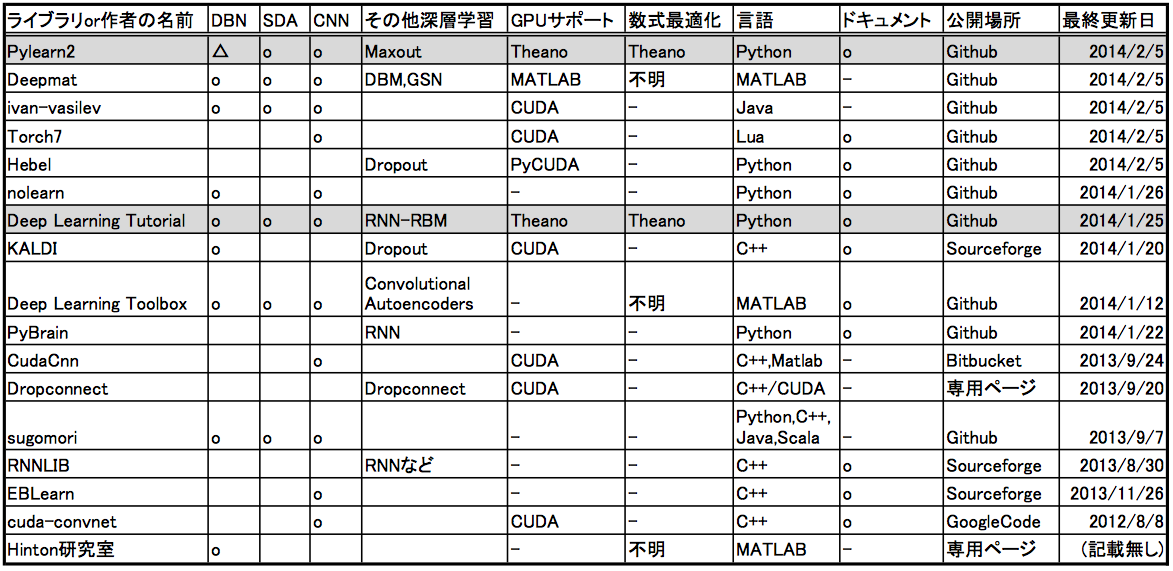
\includegraphics[width=150mm]{img/c4/dl_library}

 \label{c4_dl_library}
\end{table}

\begin{itemize}
\item \textbf{ライブラリor作者の名前} ライブラリの名前が明示されている場合はライブラリ名、そうでない場合は、作者の名前またはハンドルネームを書いた。
\item \textbf{DBN} Deep Belief Networkが実装されているかどうか。ただし、DBN自体が実装されてなくても、Deep Belief Networkの構成要素であるRBMと、pretrainingやfinetuningなど深層構造を学習するための仕組みの両方が実装されている場合は△とした。
\item \textbf{SDA} Stacked Denoising Autoencoderが実装されているかどうか。
\item \textbf{CNN} Convolutional Neural Network全体、またはConvolutional LayerとMulti Layer Perceptronを組み合わせる仕組みが実装されているかどうか。
\item \textbf{その他深層学習} その他、深層学習のアルゴリズムで実装されているもの。%略称の詳細は、各ライブラリの説明に記す。
\item \textbf{GPUサポート} GPUによる高速計算をサポートしているかどうか。
\item \textbf{数式最適化} 数式を自動で最適化し、余分な計算を省いたり、情報落ちや桁落ちを自動的に防ぐ仕組みが備わっているかどうか。ただしMATLABについては、内部的に数式を自動最適化しているかどうかに関する資料を発見できなかったため、「不明」とした。
\item \textbf{言語} ライブラリの利用者が使うプログラミング言語は何か。
\item \textbf{ドキュメント} クラス単位のドキュメントが用意されているかどうか。ここでは、サンプルコードのみが提供されている場合や、ライブラリ全体に関するドキュメントしかない場合は、「無し」に分類した。これは、「実装難易度の問題」で述べたように、ライブラリの多少の改変を視野に入れる必要からである。
\item \textbf{公開場所} ソースコードは、どのようなウェブサイトで公開されているか。
\item \textbf{最終更新日} ソースコードが最後に更新された日はいつか。
\end{itemize}

以下の項では、ここに記した深層学習ライブラリや、GPUによる高速演算をサポートするためのライブラリについて、一部紹介する。

\subsubsection{cuda-convnet}
CUDAとC++による畳み込みネットワークの実装が、CIFARデータセットの制作者であるKrizhevsky氏によって公開されている\footnote{\url{https://code.google.com/p/cuda-convnet/}}。最大値蓄積レイヤーや最終レイヤー用のソフトマックスレイヤーなど、畳み込みネットワークの実装に必要なパーツが一通り用意されている。なお、後述するPylearn2にも、このcuda-convnetのPythonラッパクラスが実装されている。
\begin{comment}
%\subsection{DropConnect}
%DropConnectのソースコードも、ウェブページにて公開されている。CUDAとC++を用いた独自のコード
%sentiment analysis

%nolearn
%deepnet
%scikit
%pycuda
\subsubsection{Hinton研究室のサンプルコード}
Matlabで書かれている
Autoencoder、classification model (???)
1.2\% 2006

\subsection{sugomoriさんのコード}
Theanoはわかりにくいので、numpyで全て書き直している。
2008年のコード準拠

\subsection{torch7}
Luaで書かれている。
Theanoとの比較表がある。
%http://torch.ch/
%http://conditional.github.io/blog/2013/12/07/an-introduction-to-torch7/
\end{comment}



\subsubsection{数値計算ライブラリTheano}
Theanoは、python上で記述される数式処理/数値計算ライブラリである。Theanoは、数式のコンパイルと実際のデータによる数値計算の2段階で動作する\cite{bergstra2010theano:}。図\ref{c4_Theano_compile}に、Theanoが動作する仕組みを示した。
\begin{figure}[tbp]
 \centering
  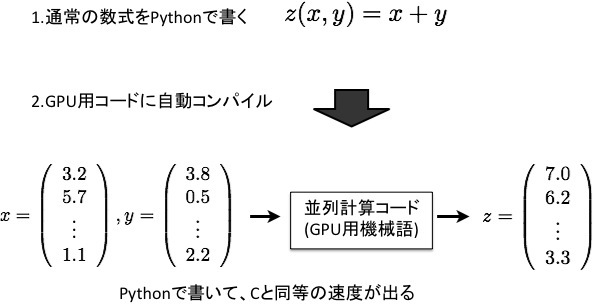
\includegraphics[width=120mm]{img/c4/theano_compile}
 \caption{Theanoの動作過程}
 \label{c4_Theano_compile}
\end{figure}
Theanoでは、数式は文字シンボルを用いた文字式で記述できる。記述された文字式は、内部的には計算木(グラフ)として蓄積されている。Theanoは、実際の計算を行う前に、このグラフをコンパイルして、CによるCUDAのコードに変換している。このときデバッグの難しい数値計算の誤差絡みの部分、0による除算など危険な処理を、自動的に解析してくれる。ニューラルネットワークの演算過程では、非常に小さい数値が出現することがあり、また、文字式を分析することで、計算グラフも最適化してくれる。プログラマは、プログラム上の些末な計算テクニックに囚われることなく、数式の本質的な部分の記述に集中することができる。また、記号ベースの解析的な微分を自動で行ってくれる機能がついている。この記号微分機能は、ニューラルネットワークの実装において大いに助けとなる。ニューラルネットワークでは、バックプロパゲーションを実装するため、モデルを構成する大量のパラメータにて、損失関数を微分する必要がある。ネットワークが多層になるとパラメータ数も増加し、微分の計算式はさらに複雑になる。微分計算を最適化するため、手計算による文字式の微分をしてから実装を行うと、層を増やす度に非常に煩雑な手計算が必要であり、開発効率の低下は避けられない。Theanoの自動微分と自動最適化は、深層学習のアルゴリズムを簡略に記述するための、大いなる助けとなる。

\subsubsection{Deep Learning Tutorial}
Deep Learning Tutorialは、Theanoを用いて記述されたソースコードで、Theanoと同じくLISA.研究室のメンバーによって書かれている。内容的には、単純なロジスティック回帰から始まり、最終的に畳み込みネットワーク, 積層雑音除去自己符号器, 深層信念ネットワークの3つの原理が理解できるよう構成されている。ソースコードのほぽ全ての部分に、詳細なコメントが書いてあり、深層学習のアルゴリズムと同時にTheanoを用いた実装上の注意点なども理解できるような作りになっている。\par
一方で、提供されているコードは簡単のため、アルゴリズムの基本的な部分に絞られており、最新の研究成果が反映されているわけではないため、注意が必要である。例えば、畳み込みネットワークのソースコードには、1998年のLeCunらによる研究\cite{lecun1998gradient-based}をベースにしていると書いてある。しかし、元の論文の段階で既に、2012年に発表された最も優れている畳み込みニューラルネットワーク\cite{ciresan2012multi-column}に比べて、3倍以上誤差が大きくなってしまっている。またあくまでTutorialという位置づけのため、繰り返し回数などのハイパーパラメータが最も誤差が低くなるようには設定されていない。\par
なお、深い構造の形にはなっていないが、雑音除去自己符号器の代わりとして、契約自己符号器\cite{rifai2011contractive}\cite{rifai2011learning}の実装も提供されている。これは、雑音除去自己符号器の亜種だが、誤差測定時に適切なベナルティ項を与えることで、学習される表現の頑健性がさらに向上するというものである。

\subsubsection{Pylearn2}
Pylearn2は、pythonで記述された、深層学習など機械学習アルゴリズムを使うためのライブラリである\cite{goodfellow2013Pylearn2:}。やはりモントリオール大学のLISA.研究室の方がメインとなっており、github上でソースコードの更新がほぼ毎日行われている。以下、Pylearn2の特徴を記す。
\begin{itemize}
\item \textbf{高精度アルゴリズムMaxout Networkの実装}
Pylearn2には、3章にて述べた、Maxout Networkという深層学習のアルゴリズムの一種が実装されている。このアルゴリズムは、画像認識タスクにおいて非常に高い精度を実現しており、高い分類精度を満たせる可能性が高い。
\item \textbf{Theanoの利用}
Pylearn2のプログラムは、前述したTheanoを全面的に利用して記述されている。Theanoを用いたことで、可読性が大きく上昇している。
\item \textbf{高度な拡張性と可読性}
Pylearn2のソースコードは、拡張性や可読性を非常に強く意識して書かれている。基本的な使い方を記したチュートリアルのウェブページが存在し、主なソースファイルには、詳細なドキュメントも記述されている。また、モジュール化が丁寧なので、自分で書く部分が少なくて済む。例えば、データセットを変更する場合は、Datasetクラスのみを書き下せばよく、他の部分に対してコードを書く必要がほとんどない。図\ref{c4_Pylearn2_yaml}に、Pylearn2において機械学習のアルゴリズムがどのようにモジュール化されているかを示す。\par
また、プログラムを改造する場合でも、数値パラメータを変更するだけであれば、設定ファイルのみの変更で完結させることができる。この設定ファイルは、YAML(YAML Ain't a Markup Language)形式に少し独自拡張を加えた形式になっている。\par
プログラム本体と、数値の設定ファイルが分離されていることで、プログラミングが不得手な人でも、比較的簡単に設定を変更することができる。\par
\begin{figure}[tbp]
 \begin{center}
  \includegraphics[width=120mm]{img/c4/Pylearn2_yaml}
 \end{center}
 \caption{Pylearn2の実験計画例}
 \label{c4_Pylearn2_yaml}
\end{figure}
\end{itemize}

\begin{comment}
\subsubsection{Pylearn2の主なパッケージ}
現在のPylearn2のソースコードは、使われているものと非推奨のものが混在している。これは、Pylearn2に定められたAPI変更のルールのためである。Pylearn2では、「変数やクラスを消去する半年前に、ライブラリ上で告知しなければならない」という管理方針を定めている。これは、Pylearn2の安定性に寄与しているが、一方で、ソースコードリーディングの際には使われていないパッケージがノイズになることも少なくない。ここでは、Pylearn2で現在使われている主なパッケージについて紹介する。
\begin{itemize}
\item \textbf{costs} 最終レイヤーで誤差を計算するときに使われる、損失関数(loss function)を集めたパッケージである。主にSGDによって利用される。Dropout、Lpペナルティ、クロスエントロピー関数、負の対数尤度関数などがここに含まれている。また、DBNや自己符号器のように、独自の損失関数が必要な場合も、ここで定義されている。
\item \textbf{datasets} MNISTやCIFAR10, SVHNなどのデータセットがクラス化されている。新しいデータセットに対して深層学習を使いたい場合は、ここに定義されているDatasetクラスやDenseDesignMatrixクラスのサブクラスを作成することになる。
\item \textbf{distributions} ガウス分布などの分布関数が集められている。
\item \textbf{gui} 主に重みフィルタを可視化するためのクラスが用意されている。
\item \textbf{linear} Theanoの線形変換クラスを作り直したもので、畳み込みレイヤーもここに含まれる。
\item \textbf{models} 自己符号器、RBMなどの学習モデルが定義されている。
\item \textbf{sandbox} cuda-convnetのラッパクラスが定義されている。
\item \textbf{scripts} 実際に学習を行わせたり、学習結果を集計するときに便利なスクリプトが集められている。
\item \textbf{train\_extensions}学習がスタートする時や、1回の処理が終了したときに動かす処理を定義するためのクラスである。デザインパターン\cite{gamma1995design}でいうObserverパターンが用いられている。
\item \textbf{training\_algorithms} SGDとバッチ勾配降下法を始めとする、学習アルゴリズムが定義されている。SGDと併用するための、学習率変化アルゴリズム(線形減少、指数関数的減少、焼き鈍し)、慣性率の利用、Polyak平均化\cite{polyak1992acceleration}なども、ここで一緒に定義されている。
\end{itemize}
\end{comment}

\subsection{深層学習ライブラリの比較と選定}
表\ref{c4_dl_library}において、「学習時間の問題」を解決するのに役立つ項目が、"GPUサポート"である。また、「実装難易度の問題」を解決するのに役立つ項目が、"数式最適化"、"ドキュメント"である。「分類精度の再現の問題」については、実際に再現実験を行わないと評価できないため、ここでは扱わない。また、3つの問題に比べれば優先度はかなり落ちるが、以下の点も考慮に値する。
\begin{itemize}
\item \textbf{実装されているモデルの豊富さ}。具体的には、"DBN"、"SDA"、"CNN"、"その他深層学習"の欄である。これが多ければ、より様々な実験が行いやすくなる。
\item \textbf{開発の活発さ}。これは、"公開場所"、"最終更新日"の欄が当てはまる。開発が活発ならば、ライブラリの使用で問題が起きたとき、他の開発コミュニティのメンバーから助けてもらえる可能性が高くなる。また、最新の研究結果がライブラリに取り込まれる可能性も出てくる。Githubを始めとするオープンな開発が行われている場所に公開されているコードは、より多くの人によって開発が進行する可能性が高い。また、最終更新日が新しければ、開発がストップしてしまっていないことの証になる。
\end{itemize}
以上の要素を同時に満たしているライブラリは、Pylearn2とDeep Learning Tutorialのみである。また、この2つのライブラリは、DBN・SDA・CNNという深層学習の主要なアルゴリズムをほぼ網羅している。さらに、Pylearn2にはMaxout Networkという深層学習のアルゴリズムが実装されている。これは、MNISTの順序不変タスクにて最先端の精度を達成したアルゴリズムであり、Pylearn2を使うことは分類性能面でも期待できる。\par
深層学習にて、冒頭に挙げた3つの問題点のうち、「学習時間の問題」「実装難易度の問題」の2つは、Pylearn2もしくはDeep Learning Tutorialというライブラリをベースに実装を進めることで、解決できると言える。残る「分類性能の再現の問題」については、実際に実験を行って精度を測定した上で、再現が出来ているかどうかチェックすることになる。

\section{結論}
この章では、深層学習のアルゴリズムの実装上の3つの問題点を挙げた後、その対策について述べた。ソフトウェア面では、深層学習のライブラリであるPylearn2もしくはDeep Learning Tutorialの使用が、問題点のうち2つを解決できる点で望ましいことを示した。ただし、「分類性能の再現の問題」については、5章にて実際に分類精度の再現実験を行った後判断する必要がある。また、ハードウェア面では、実験に使うマシンに、NVIDIA社のGeForceシリーズに属するGPUで、GTX280以上のバージョンのものを搭載することで、「学習時間の問題」を大きく緩和できることがわかった。